\documentclass[tikz,border=2mm,landscape,12pt]{standalone}
\usepackage{tikz}
\usepackage{kotex}
\usetikzlibrary{shapes.misc, positioning}
\renewcommand{\familydefault}{\sfdefault}

\begin{document}
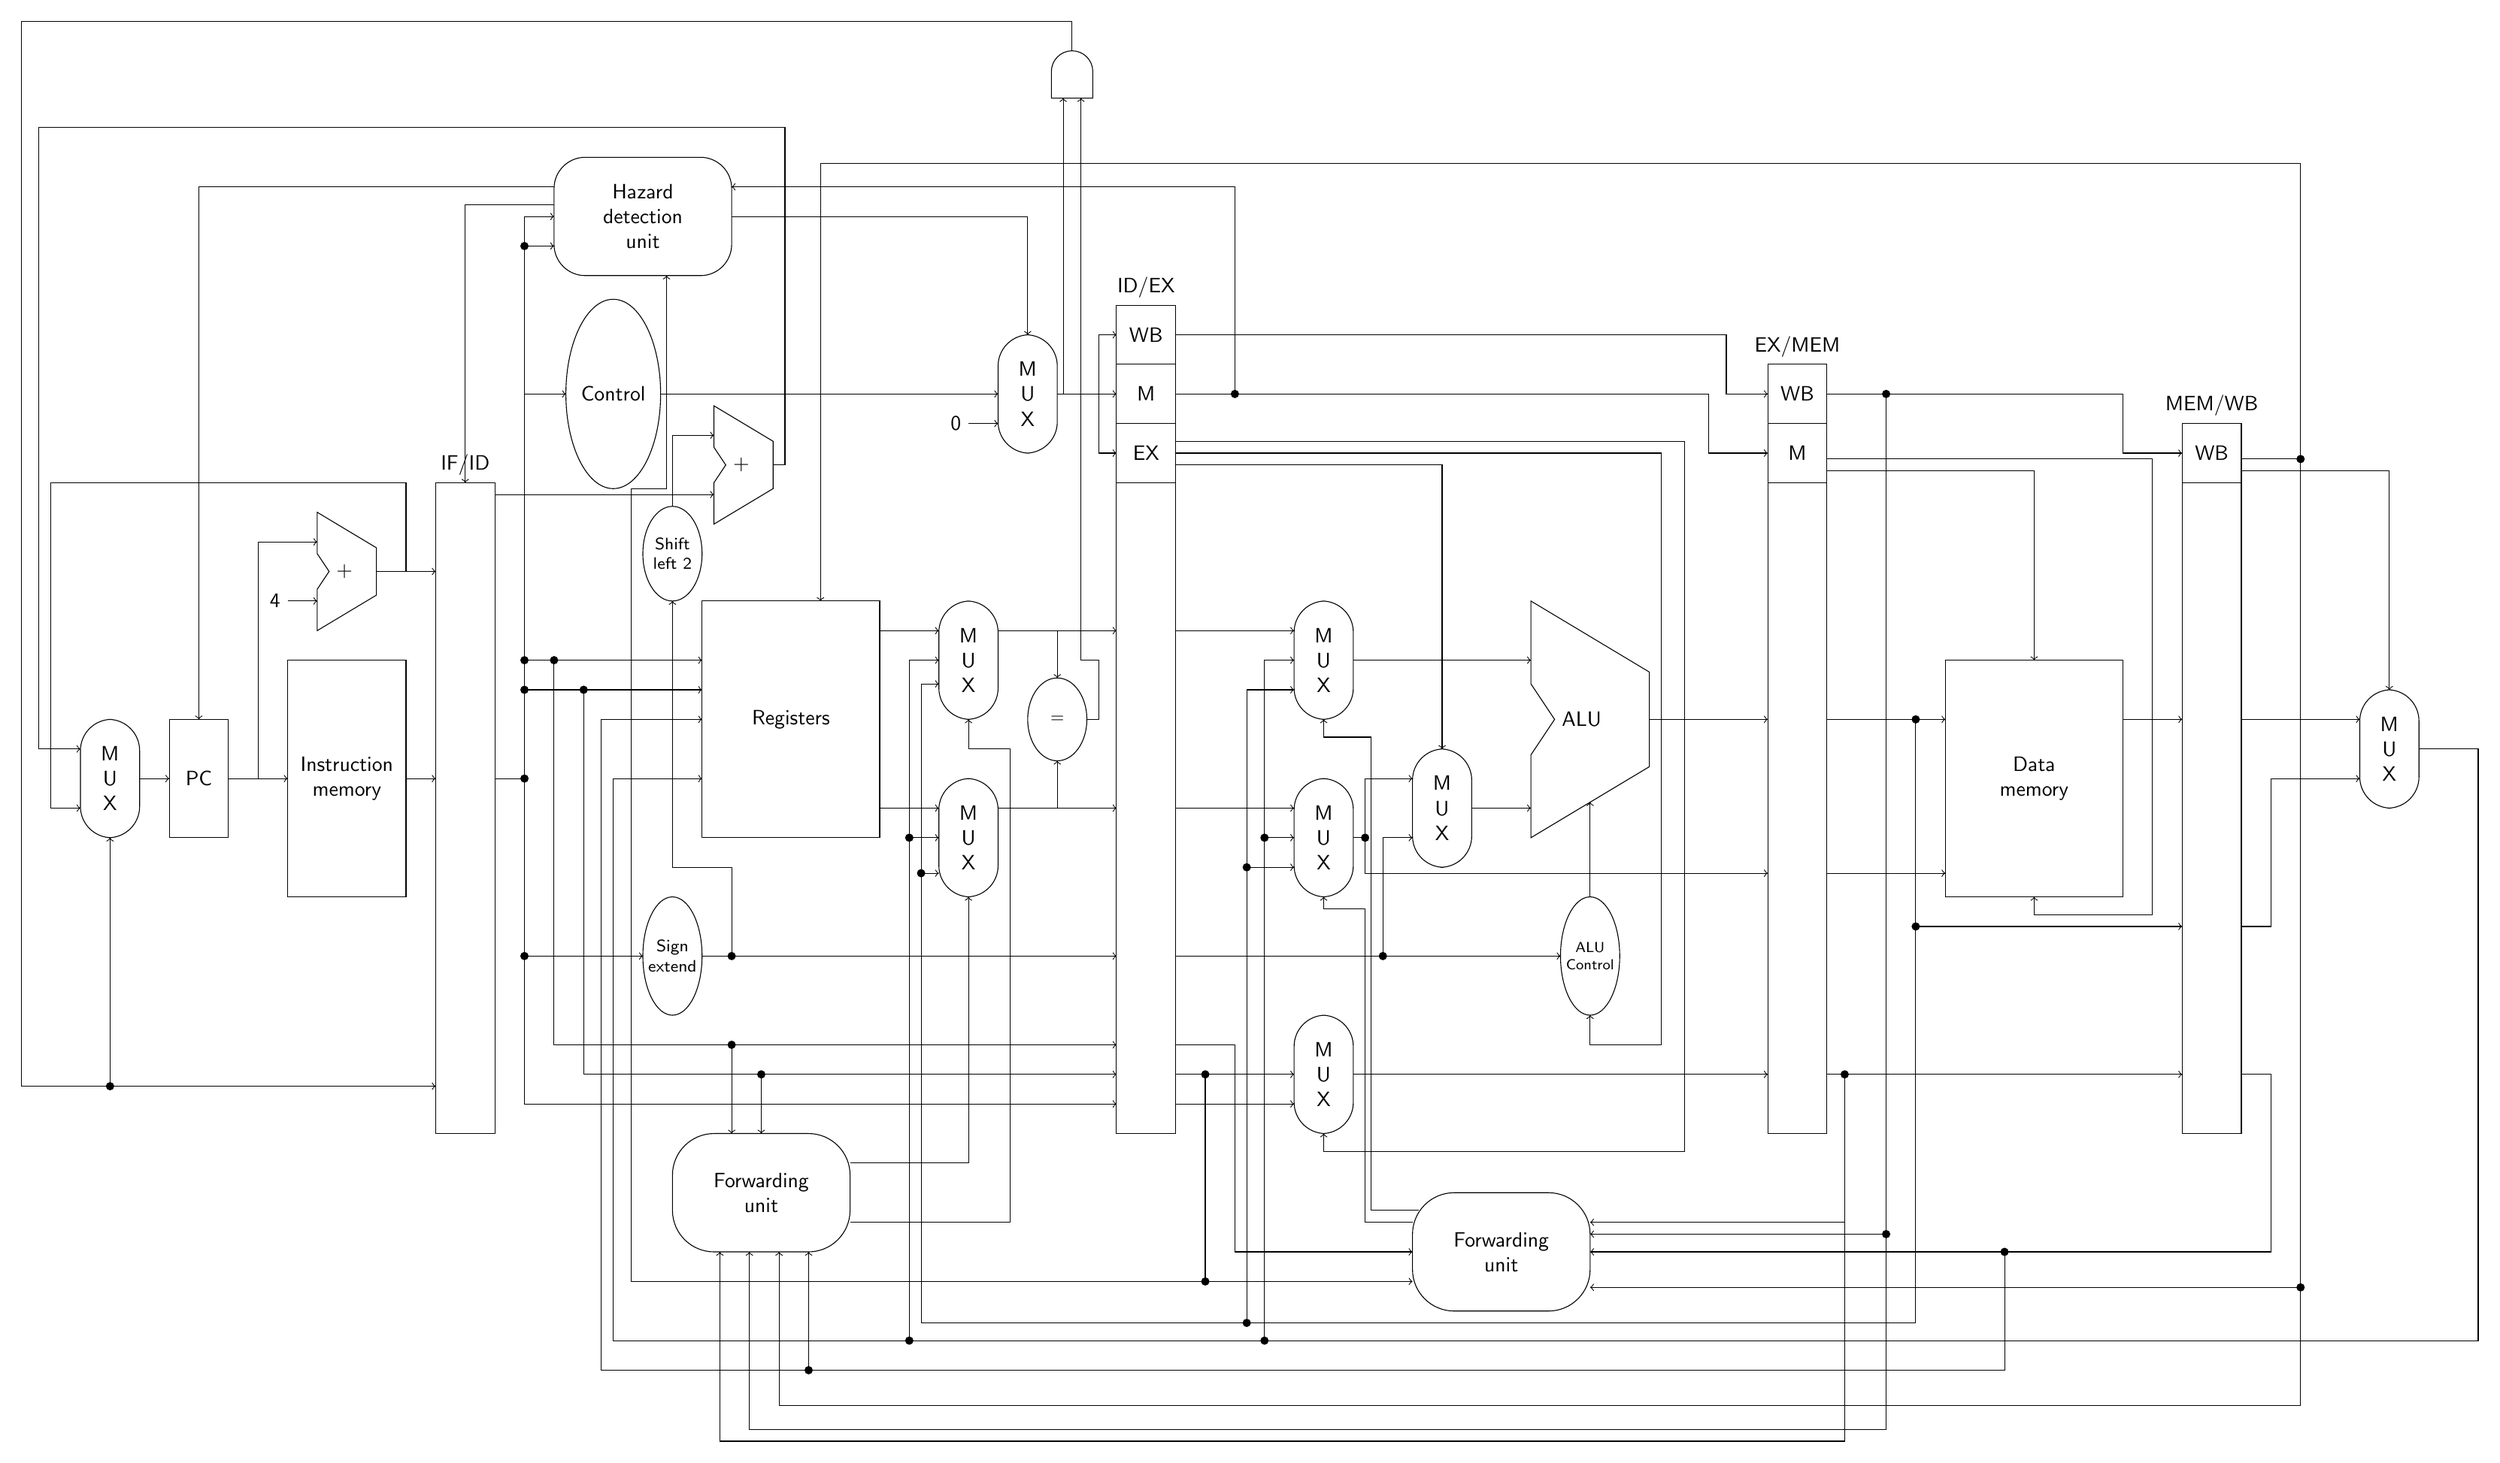
\begin{tikzpicture}
\tikzset{rs/.style}
\tikzset{rt/.style}
\tikzset{rd/.style}
\tikzset{immed/.style}
\tikzset{addr/.style}

% Instruction Fetch
\begin{scope}
    \draw[rounded corners=15pt] (-1.5,0) rectangle ++(1,2);
    \node[align=center] at (-1, 1) {M \\ U \\ X};
    \draw (0,0) rectangle (1,2) node[pos=.5] {PC};
    \draw (2,-1) rectangle (4,3) node[pos=.5, align=center] {Instruction \\ memory};

    \draw (2.5,3.5) --++(0,0.7) --++(0.2,0.3) node[right] {+} --++(-0.2,0.3) --++(0,0.7) --++(1,-0.6) --++(0,-0.8) -- cycle;
    \draw[->] (1,1) --++(1,0);
    \draw[->] (4,1) --++(0.5,0);
    \draw[->] (1.5,1) --++(0,4) --+(1,0);
    \draw[->] (2,4) node[left] {4} --++(0.5,0);
    \draw[->] (3.5,4.5) --++(1,0);
    \draw[->] (4,4.5) --++(0,1.5) --++(-6,0) --++(0,-5.5) --++(0.5,0);
    \draw[->] (-0.5,1) --++(0.5,0);
\end{scope}

%Instruction Decode
\begin{scope}[xshift=3.5cm,on grid]
    % dot
    \foreach \x/\y in {2.5/-2, 3/3, 3.5/2.5, 6/-2, -4.5/-4.2, 2.5/1, 2.5/2.5, 2.5/3, 2.5/10, 6/-3.5, 6.5/-4}
    \fill (\x,\y) circle(2pt);

    % IF/ID
    \draw (1,-5) rectangle (2,6);
    \node[above] at (1.5,6) {IF/ID};

    % Register
    \draw (5.5,0) rectangle (8.5,4) node[pos=.5] {Registers};
    \draw[rs, rt, rd] (2,1) --++(0.5,0);
    \draw[rs, ->] (2.5,1) --++(0,2) --++(3,0);
    \draw[rt, ->] (2.5,1) --++(0,1.5) --++(3,0);

    % Control
    \draw (4,7.5) ellipse (0.8 and 1.6);
    \node[align=center] at (4,7.5) {Control};

    \draw[->] (2.5,7.5) --++(0.7,0);
    \draw[->] (4.8,7.5) --++(5.7,0);

    % MUX Control
    \draw[rounded corners=15pt] (10.5,6.5) rectangle ++(1,2);
    \node[align=center] at (11, 7.5) {M \\ U \\ X};
    \draw[->] (10,7) --++(0.5,0);
    \node[left] at (10,7) {0};
    \draw[->] (11.5,7.5) --++(1,0);
    \draw[->] (12.2,7.5) --++(0,1) --++(0.3,0);
    \draw[->] (12.2,7.5) --++(0,-1) --++(0.3,0);
    \draw[->] (11.6,7.5) --++(0,5);

    % Hazard Detection Unit
    \draw[rounded corners=15pt] (3,9.5) rectangle ++(3,2);
    \node[align=center] at (4.5,10.5) {Hazard \\ detection \\ unit};
    \draw[rs, ->] (2.5,1) --++(0,9) --++(0.5,0);
    \draw[rs, ->] (2.5,10) --++(0,0.5) --++(0.5,0);
    \draw[->] (6,10.5) --++(5,0) --++(0,-2); % to Control Mux
    \draw[->] (3,10.7) --++(-1.5,0) --++(0,-4.7); % IF/IDWrite
    \draw[->] (3,11) --++(-6,0) --++(0,-9); % PCWrite

    % Sign Extend
    \draw (5,-2) ellipse (0.5 and 1);
    \node[align=center, font=\footnotesize] at (5,-2) {Sign \\ extend};
    \draw[immed, ->] (2.5,1) --++(0,-3) --++(2,0);
    \draw[immed, ->] (5.5,-2) --(12.5,-2);
    \draw[immed, ->] (6, -2) --++(0,1.5) --++(-1,0) --++(0,4.5);

    % Shift Left 2
    \draw (5, 4.8) ellipse (0.5 and 0.8);
    \node[align=center, font=\footnotesize] at (5,4.8) {Shift \\ left 2};
    \draw[->] (2, 5.8) --++(3.7,0);
    \draw[->] (5,5.6) --++(0,1.2) --++(0.7,0);

    % +
    \draw (5.7,5.3) --++(0,0.7) --++(0.2,0.3) node[right] {+} --++(-0.2,0.3) --++(0,0.7) --++(1,-0.6) --++(0,-0.8) -- cycle;
    \draw[->] (6.7,6.3) --++(0.2,0) --++(0,5.7) --++(-12.6,0) --++(0, -10.5) --++(0.7,0);

    % MUX rs
    \draw[rounded corners=15pt] (9.5,2) rectangle ++(1,2);
    \node[align=center] at (10,3) {M \\ U \\ X};
    \draw[rs, ->] (8.5,3.5) --++(1,0);
    \draw[rs, ->] (10.5,3.5) --++(2,0);
    
    % MUX rt
    \draw[rounded corners=15pt] (9.5,-1) rectangle ++(1,2);
    \node[align=center] at (10,0) {M \\ U \\ X};
    \draw[rt, ->] (8.5,0.5) --++(1,0);
    \draw[rt, ->] (10.5,0.5) --++(2,0);

    % =
    \draw (11.5,2) ellipse (0.5 and 0.7);
    \node[align=center, font=\footnotesize] at (11.5,2) {=};
    \draw[->] (11.5,3.5) --++(0,-0.8);
    \draw[->] (11.5,0.5) --++(0,0.8);
    \draw[->] (12,2) --++(0.2,0) --++(0,1) --++(-0.3,0) --++(0,9.5);

    % Forwarding Unit
    \draw[rounded corners=20pt] (5,-7) rectangle ++(3,2);
    \node[align=center] at (6.5,-6) {Forwarding \\ unit};
    \draw[rs, ->] (6,-3.5) --++(0,-1.5);
    \draw[rt, ->] (6.5,-4) --++(0,-1);
    \draw[->] (8,-5.5) --++(2,0) --++(0,4.5);
    \draw[->] (8,-6.5) --++(2.7,0) --++(0,8) --++(-0.7,0) --++(0,0.5);

    % IF.Flush
    \draw (11.4,12.5) {[rounded corners=10pt] --++(0,0.8) --++(0.7,0)} --++(0,-0.8) --cycle;
    \draw[->] (11.75,13.3) --++(0,0.5) --++(-17.75,0) --++(0,-18) --++(7,0);
    \draw[->] (-4.5, -4.2) --++(0,4.2); % to IF PCSrc

    % rs, rt, rd to ID/EX
    \draw[rd, ->] (2.5,-2) --++(0,-2.5) --++(10,0);
    \draw[rs, ->] (3,3) --++(0,-6.5) --++(9.5,0); 
    \draw[rt, ->] (3.5,2.5) --++(0,-6.5) --++(9,0);
\end{scope}

% Execution
\begin{scope}[xshift=16cm]
    % dot
    \foreach \x/\y in {2.2/-0.5, 4.5/-2, 1.5/-7.5, 1.5/-4, 2/7.5, 4.2/0} % 6.5/0.5
    \fill (\x,\y) circle(2pt);

    % ID/EX
    \draw (0,-5) rectangle (1,6);
    \draw (0,6) rectangle ++(1,1) node[pos=.5]{EX};
    \draw (0,7) rectangle ++(1,1) node[pos=.5]{M};
    \draw (0,8) rectangle ++(1,1) node[pos=.5]{WB};
    \node[above] at (0.5,9) {ID/EX};

    \draw[->] (1,8.5) --++(9.3,0) --++(0,-1) --++(0.7,0); % WB Control
    \draw[->] (1,7.5) --++(9,0) --++(0,-1) --++(1,0); % M Control
    \draw[->] (2,7.5) --++(0,3.5) --++(-8.5,0); % MemRead to Hazard Detection Unit
    \draw[->] (1,6.3) --++(4.5,0) --++(0,-4.8); % ALUSrc
    \draw[->] (1,6.5) --++(8.2,0) --++(0,-10) --++(-1.2,0) --++(0,0.5); % ALUOp
    \draw[->] (1,6.7) --++(8.6,0) --++(0,-12) --++(-6.1,0) --++(0,0.3); % RegDst

    % ALU
    \draw (7,0) --++(0,1.4) --++(0.4,0.6) node[right] {ALU} --++(-0.4,0.6) --++(0,1.4) --++(2,-1.2) --++(0,-1.6) -- cycle;
    \draw[->] (9,2) --++(2,0);

    % Forwarding Unit
    \draw[rounded corners=20pt] (5,-8) rectangle ++(3,2);
    \node[align=center] at (6.5,-7) {Forwarding \\ unit};
    \draw[rs, ->] (1,-3.5) --++(1,0) --++(0,-3.5) --++(3,0); % EX.rs
    \draw[rt, ->] (1,-4) --++(0.5,0) --++(0,-3.5) --++(3.5,0); % EX.rt
    \draw[->] (5.1,-6.3) --++(-0.8,0) --++(0,8) --++(-0.8,0) --++(0,0.3); % ForwardA
    \draw[->] (5,-6.5) --++(-0.8,0) --++(0,5.3) --++(-0.7,0) --++(0,0.2); % ForwardB
    
    % MUX above
    \draw[rounded corners=15pt] (3,2) rectangle ++(1,2);
    \node[align=center] at (3.5,3) {M \\ U \\ X};
    \draw[rs, ->] (1,3.5) --++(2,0);
    \draw[->] (4,3) --++(3,0);

    % MUX below
    \draw[rounded corners=15pt] (3,-1) rectangle ++(1,2);
    \node[align=center] at (3.5,0) {M \\ U \\ X};
    \draw[rt, ->] (1,0.5) --++(2,0);
    \draw[->] (4,0) --++(0.2,0) --++(0,1) --++(0.8,0);
    \draw[->] (4.2,0) --++(0,-0.6) --++(6.8,0);
    
    % MUX ALUsrc
    \draw[rounded corners=15pt] (5,-0.5) rectangle ++(1,2);
    \node[align=center] at (5.5,0.5) {M \\ U \\ X};
    \draw[->] (1,-2) --++(3.5,0) --++(0,2) --++(0.5,0);
    \draw[->] (6,0.5) --++(1,0);
    % \draw[->] (6.5,0.5) --++(0,-1) --++(4.5,0); % IS IT CORRECT?
    
    % MUX RegDst
    \draw[rounded corners=15pt] (3,-5) rectangle ++(1,2);
    \node[align=center] at (3.5,-4) {M \\ U \\ X};
    \draw[rt, ->] (1,-4) --++(2,0);
    \draw[rd, ->] (1,-4.5) --++(2,0);
    \draw[->] (4,-4) --++(7,0);

    % ALU Control
    \draw (8,-2) ellipse (0.5 and 1);
    \node[align=center, font=\scriptsize] at (8,-2) {ALU \\ Control};
    \draw[->] (1,-2) --++(6.5,0);
    \draw[->] (8,-1) --++(0,1.6);

    % rt to Hazard detection unit
    \draw[rd, ->] (1.5,-7.5) --++(-9.7,0) --++(0,13.4) --++(0.6,0) --++(0,3.6);

\end{scope}

% MEM
\begin{scope}[xshift=27cm]
    % dot
    \foreach \x/\y in {2.5/2, 2.5/-1.5, 1.3/-4, 2/7.5, 2/-6.7, -8.8/-8.2, -14.3/-0.6}
    \fill (\x,\y) circle(2pt);

    % EX/MEM
    \draw (0,-5) rectangle (1,6);
    \draw (0,6) rectangle ++(1,1) node[pos=.5]{M};
    \draw (0,7) rectangle ++(1,1) node[pos=.5]{WB};
    \node[above] at (0.5,8) {EX/MEM};

    \draw[->] (1,7.5) --++(1,0) --++(0,-14.2) --++(-5,0); % RegWrite to Forwarding Unit (EX)
    \draw[->] (2,-6.7) --++(0,-3.3) --++(-19.2,0) --++(0,3); % RegWrite to Forwarding Unit (ID)
    \draw[->] (2,7.5) --++(4,0) --++(0,-1) --++(1,0); % RegWrite to MEM/WB
    \draw[->] (1,6.4) --++(5.5,0) --++(0,-7.7) --++(-2,0) --++(0,0.3); % MemRead
    \draw[->] (1,6.2) --++(3.5,0) --++(0,-3.2); % MemWrite
    
    % Memory
    \draw (3,-1) rectangle ++(3,4) node[pos=.5, align=center] {Data \\ memory};
    \draw[->] (1,2) --++(2,0); % Addr
    \draw[->] (1,-0.6) --++(2,0); % WriteData
    \draw[->] (6,2) --++(1,0); % ReadData

    \draw[->] (2.5,2) --++(0,-3.5) --++(4.5,0);
    % ALU Result Forwarding (EX)
    \draw[->] (2.5,-1.5) --++(0,-6.7) --++(-11.3,0) --++(0,10.7) --++(0.8,0);
    \draw[->] (-8.8,-0.5) --++(0.8,0);
    % ALU Result Forwarding (ID)
    \draw[->] (-8.8,-8.2) --++(-5.5,0) --++(0,10.8) --++(0.3,0);
    \draw[->] (-14.3,-0.6) --++(0.3,0);

    % RegDst
    \draw[->] (1,-4) --++(6,0);
    \draw[->] (1.3,-4) --++(0,-2.5) --++(-4.3,0); % Forwarding Unit (EX)
    \draw[->] (1.3,-6.5) --++(0,-3.7) --++(-19,0) --++(0,3.2); % Forwarding Unit (ID)


\end{scope}

% WB
\begin{scope}[xshift=34cm]
    % dot
    \foreach \x/\y in {2/6.4, -3/-7, -15.5/-8.5, -15.5/0, 2/-7.6, -23.2/-9, -21.5/0, -21.5/-8.5}
    \fill (\x,\y) circle(2pt);

    % MEM/WB
    \draw (0,-5) rectangle (1,6);
    \draw (0,6) rectangle ++(1,1) node[pos=.5]{WB};
    \node[above] at (0.5,7) {MEM/WB};

    \draw[->] (1,6.2) --++(2.5,0) --(3.5,2.5); % MemtoReg
    \draw[->] (1,6.4) --++(1,0) --++(0,-14) --++(-12,0); % RegWrite to Forwarding Unit (EX)
    \draw[->] (2, -7.6) --++(0,-2) --++(-25.7,0) --++(0,2.6); % RegWrite to Forwarding Unit (ID)
    \draw[->] (2,6.4) --++(0,5) --++(-25,0) --++(0,-7.4); % RegWrite to Register

    % MUX Writedata
    \draw[rounded corners=15pt] (3,0.5) rectangle ++(1,2);
    \node[align=center] at (3.5,1.5) {M \\ U \\ X};
    \draw[->] (1,2) --++(2,0);
    \draw[->] (1,-1.5) --++(0.5,0) --++(0,2.5) --++(1.5,0);

    % RegDst
    \draw[->] (-3,-7) --++(0,-2) --++(-23.7,0) --++(0,11) --++(1.7,0); % to Register
    \draw[->] (1,-4) --++(0.5,0) --++(0,-3) --++(-11.5,0); % to Forwarding Unit (EX)
    \draw[->] (-23.2,-9) --++(0,2); % to Forwarding Unit (ID)

    % Write Data!
    \draw[->] (-15.5,-8.5) --++(-11,0) --++(0,9.5) --++(1.5,0); % to Register
    \draw[->] (4,1.5) --++(1,0) --++(0,-10) --++(-20.5,0) --++(0,11.5) --++(0.5,0); % to EX above MUX
    \draw[->] (-15.5,0) --++(0.5,0); % to EX below MUX
    \draw[->] (-21.5,-8.5) --++(0,11.5) --++(0.5,0); % to ID upper MUX
    \draw[->] (-21.5,0) --++(0.5,0); % to ID below MUX
\end{scope}
\end{tikzpicture}

\end{document}